Although Bitcoin stores all the transactions in a public
ledger accessible to everyone, it is not always easy to trace
the ownership back to a real person. Also, there are steps
one can take to prevent being detected by the network
analysis techniques. As long as protocol level anonymity is built around Bitcoin, there are several workarounds that one
can follow to hide one's true identity. Any user not taking proactive steps to conceal himself is at a high risk of being
found.

\section{Be careful of Bitcoin Exchanges}
While buying Bitcoins, do not buy them from MtGox, Coinbase or other exchanges that need your bank account and ask you
for your name. Instead, one can mine them from a Bitcoin pool
like Eligius (no accounts/email necessary, they only ask for
a bitcoin address) \cite{eli}. Doing so covers one weak point
of Bitcoin in that the identity of the owner at the point of
origin of the coin is protected.

\section{Zerocoin}
After getting the Bitcoins, before spending them, one can pass them through several intermediate services to mask their point of origin. One such service is Zerocoin \cite{zero}. 
Zerocoin is a distributed e-cash scheme that aims to keep Bitcoin anonymous by using cryptographic techniques. A user takes his Bitcoins and converts them into Zerocoins. This
takes the Bitcoins out of the public ledger. Payments can now
be made via Zerocoins to other users, and split and merge
Zerocoins in any way that preserves its total value. By
reconverting Zerocoins to Bitcoins, a new private-public key pair is generated thus breaking the link in the block chain.
\\*
\begin{center}
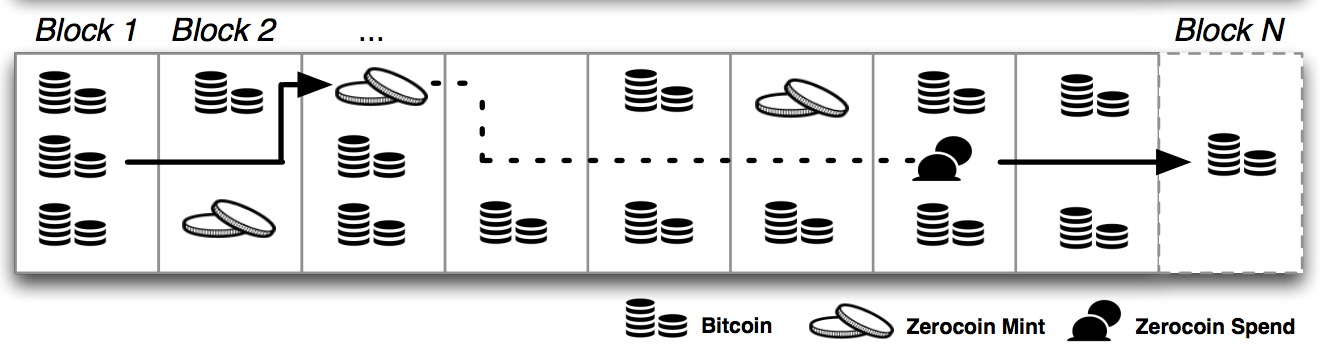
\includegraphics[scale=0.5]{images/zero.png}
\end{center}

\section{For the Paranoid User}
\subsection{Anonymous Hardware and Software}
For users who are serious about protecting their identity, it is necessary to use anonymous hardware. One can buy a cheap laptop and remove its hard drive. It is important that one does not connect it to the home wifi that can be traced back to him. For the next step, the user can download a Linux LiveCD to connect to the TOR network /cite{paranoid}. 

\subsection{Create an anonymous wallet}
Do not use any eWallet to store your Bitcoins. Apart from being insecure, some of the wallets themselves are fraud or ponzi schemes to steal user’s Bitcoins. Instead, use a service like BitAddress \cite{bitaddress} that can be used to generate Bitcoin addresses offline. Also, the addresses and private key pair generated allows one to spend and receive Bitcoins without running any other external software.

\subsection{Funding the anonymous wallet}
This step refers to filling one’s wallet with Bitcoins and is arguably the most difficult step. One must take extra care not buy Bitcoins from banks or Bitcoin Exchanges as they are easy to trace. Instead, one can exchange cash for Bitcoins from cash transaction networks like ZipZap \cite{zip} that do not verify the buyer’s identity. One can provide a fake email address for the purchase.

\subsection{Spending your Bitcoins}
Before spending the Bitcoins you have, you should send the
funds through a mixing service that mixes one’s Bitcoins with
others to confuse anyone following the trail \cite{mix}.
However, an important point to note here that the mixing
services are not always trustworthy and may steal your money.
Instead one can use services such as Zerocoin(as mentioned
above) to do the mixing. Also, these mixing wallets should
not be created using the TOR network as the TOR exit node may
be monitored. In a yet to be published paper researchers from
Cornell University argue that the TOR network is susceptible
to man-in-the-middle attacks thus affecting Bitcoin’s privacy
as well~\cite{badidea}.







